%% ============================================================================
%% CCF-GNN — Springer Nature journal article (sn-jnl class)
%% ----------------------------------------------------------------------------
%% Compile: pdflatex main && bibtex main && pdflatex main && pdflatex main
%% Requires sn-jnl.cls and sn-basic.bst in the same folder (Springer Nature
%% LaTeX template, https://www.springernature.com/gp/authors/campaigns/latex-author-support)
%%
%% HONESTY NOTES FOR THE AUTHORS (delete before submission):
%%  * Every number marked \tbd{...} MUST be replaced by results from the full
%%    protocol (experiments/README.md). Do not submit with red placeholders.
%%  * Tables in tables/ are auto-generated from real runs by
%%    experiments/make_tables.py — do not edit them by hand.
%%  * Fill author/affiliation/funding details.
%% ============================================================================
\documentclass[pdflatex,sn-basic]{sn-jnl}

\usepackage{graphicx}
\usepackage{multirow}
\usepackage{amsmath,amssymb,amsfonts}
\usepackage{amsthm}
\usepackage{booktabs}
\usepackage{xcolor}

\newtheorem{proposition}{Proposition}
\newtheorem{remark}{Remark}

\newcommand{\tbd}[1]{\textcolor{red}{\textbf{[#1]}}}          % placeholder: replace before submission
\newcommand{\Ac}{\mathbf{A}_{\mathrm{CCF}}}
\newcommand{\Ah}{\mathbf{A}_{\mathrm{hyb}}}
\newcommand{\Ahi}{\mathbf{A}_{\mathrm{hyb},ij}}
\newcommand{\Ar}{\mathbf{A}_{\mathrm{res}}}
\newcommand{\R}{\mathbb{R}}

\raggedbottom

\begin{document}

\title[CCF-GNN: Auditing Time-Lagged Correlation Graphs for Traffic Forecasting]{How Reliable Are Time-Lagged Correlation Graphs for Traffic Forecasting? An Empirical Audit and the Screened-Hybrid CCF-GNN}

\author*[1]{\fnm{Morteza} \sur{Farid Agh Ghaleh}}\email{morteza.farid.a@gmail.com}
\equalcont{These authors contributed equally to this work.}
\author[1]{\fnm{Ebrahim} \sur{Akbari}}
\equalcont{These authors contributed equally to this work.}
\author[1]{\fnm{Homayoon} \sur{Motameni}}

\affil*[1]{\orgdiv{Faculty of Computer Science}, \orgname{Islamic Azad University, Sari Branch}, \orgaddress{\city{Sari}, \country{Iran}}}

\abstract{The graphs that drive spatio-temporal graph neural networks for traffic forecasting are
routinely built from pairwise, time-lagged correlations, yet their actual reliability has never
been quantified. We audit this construction on the standard METR-LA benchmark and find that raw
significance testing is nearly vacuous (93--98\% of directed sensor pairs pass at $p<0.05$),
that the effect-size threshold is the binding constraint, and that only about 23\% of surviving
edges are physically compatible with propagation over road distances. Because real benchmarks
carry no ground-truth causal graph, we add a calibrated synthetic benchmark---207 nodes on the
real road topology, 725 true time-lagged edges, latent confounders---on which significance-only
admission yields $1.7\%$ precision, the effect-size screen removes ${\sim}90\%$ of false
edges, and the fully screened deployed graph reaches $28.6{\pm}1.6\%$ precision at
$57{\pm}3\%$ recall, while estimated propagation lags are exact in ${\sim}99.5\%$ of
recovered edges. Motivated by this audit, CCF-GNN consumes the screened graph through a masked
hybrid adjacency with per-edge gates initialised by validation status, aligns graph convolution
with the estimated lags, and emits deterministic, template-based explanations restricted to
validated tuples---read as screened hypotheses, not verified mechanisms. In same-budget comparisons on real data
(25\% of training windows, CPU), CCF-GNN clearly beats the historical average and improves over
a same-budget Graph WaveNet by $14.2\%$ MAE at 15\,min and $7.4\%$ at 30\,min, while conceding
$3.4\%$ at 60\,min---a horizon-dependent profile consistent with its audit-based design intent;
under random sensor masking of up to 15\% of nodes both models degrade by at most ${\sim}4\%$
relative MAE and CCF-GNN's absolute error remains the lower one at every level. We claim no
accuracy record: the contribution is the audited, screened structure and its grounded
explanations. Every reported number is generated by script from released
code and seeds.}

\keywords{Traffic forecasting, Graph neural networks, Granger causality, Cross-correlation,
Explainability, Intelligent transportation systems}

\maketitle

\section{Introduction}\label{sec:intro}

Short-term traffic forecasting is a core component of intelligent transportation systems (ITS),
supporting proactive congestion management, adaptive ramp metering, and traveller information.
The task is governed by a distinctive physical mechanism: a disturbance at an upstream location
propagates to downstream locations after a travel-time delay that varies with the traffic regime
\cite{may1990,lighthill1955,richards1956}. Spatio-temporal graph neural networks (STGNNs)
\cite{li2019dcrnn,yu2019stgcn,wu2019gwn,wu2020mtgnn} dominate the leaderboards by coupling graph
convolutions over a road or learned graph with temporal encoders. Their success, however, rests
on graph structures that are either fixed and purely geographic---hence blind to non-local
functional dependencies---or learned end-to-end and therefore opaque: an edge in a learned
adjacency matrix has no inspectable semantics, no direction justified by data, and no notion of
propagation delay.

This opacity matters operationally. Traffic management centres do not merely ask \emph{what} the
speed will be in one hour; they ask \emph{which} upstream corridors are driving the predicted
congestion, \emph{how soon} the influence arrives, and \emph{how much} the prediction depends on
a sensor that is about to fail. Post-hoc explanation tools (attention visualisation, gradient
attribution, GNNExplainer-style masking) answer none of these questions reliably: attention
weights do not imply causation \cite{rudin2019}, gradients are unstable under saturation
\cite{sundararajan2017}, and post-hoc explainers faithfully extract spurious patterns when the
underlying model learned them \cite{ying2019gnnexplainer,yuan2021subgraphx}.

Four gaps in the literature motivate this work:
\begin{enumerate}
\item \textbf{Time-lag ignorance.} Mainstream STGNNs treat spatial edges as instantaneous; the
physical delay structure of propagation is at best implicit in recurrent state.
PDFormer \cite{xu2024pdformer} attends to time-shifted features but derives delays implicitly
inside the attention mechanism, without statistical validation or inspectable semantics.
\item \textbf{Structural opacity.} Adaptive graphs \cite{wu2019gwn,bai2020agcrn,wu2020mtgnn}
achieve accuracy at the cost of black-box structure.
\item \textbf{Post-hoc explanation limits.} Existing explainers identify correlations rather than
validated temporal dependencies and add per-query computational overhead
\cite{ying2019gnnexplainer,yuan2021subgraphx,lundberg2017,ribeiro2016}.
\item \textbf{Causality used in isolation.} Applications of Granger causality in transportation
typically stop at discovery, using the causal graph as a static input to a separate predictor and
without addressing stationarity, confounding, or explanation generation
\cite{liu2022metro}.
\end{enumerate}

\subsection{Contributions}\label{sec:contrib}

We propose \textbf{CCF-GNN}, a framework in which the propagation delay is a first-class,
interpretable component of both the graph and the explanation. Our contributions are:

\begin{itemize}
\item \textbf{C1 --- An empirical audit of lagged-correlation graph construction.} On real
METR-LA: significance vacuity, effect-size dominance, and physical infeasibility of most raw
edges; on a calibrated synthetic benchmark with known ground truth: stage-by-stage recovery
quantifying exactly what each screening stage buys (Table~\ref{tab:synthetic}).
\item \textbf{C2 --- A reproducible screening pipeline.} Effect-size threshold, Benjamini--Hochberg
FDR control, path-based confounding screen, physical-feasibility check, and degree cap ---
released as code and characterised by C1.
\item \textbf{C3 --- CCF-GNN.} A masked hybrid adjacency that keeps the screened prior fixed and
fuses it with a learnable residual through per-edge gates initialised by validation status,
combined with a lag-aligned graph convolution.
\item \textbf{C4 --- A grounded intrinsic explainer.} Deterministic Top-$K$ extraction over a
single importance score, fixed natural-language templates, and rule-based validity checks;
explanations are deterministic, traceable, and explicitly scoped as screened hypotheses.
\item \textbf{C5 --- A fully reproducible evaluation protocol.} Masked DCRNN-style metrics,
fixed seeds, script-generated tables, honestly scoped medium- and reduced-scale comparisons on
real data (including a real sensor-masking robustness study), and released generator code for
the synthetic ground-truth study.
\end{itemize}

\subsection{Scope of causal claims}\label{sec:scope}

Throughout, ``causal'' means \emph{Granger-type predictive causality}: past values of $x_j$
carry statistically non-trivial information about future values of $x_i$
\cite{granger1969}. We do not claim interventional (do-calculus) causality
\cite{pearl2009,peters2017}; the confounding screen provides evidence \emph{against} the most
common failure mode, not proof of mechanism. Section~\ref{sec:discussion} returns to this point.

\section{Related work}\label{sec:related}

\subsection{Spatio-temporal graph neural networks}
DCRNN \cite{li2019dcrnn} recasts traffic forecasting as sequence-to-sequence diffusion
convolution over a distance-thresholded road graph; STGCN \cite{yu2019stgcn} replaces recurrence
with temporal convolution. Graph WaveNet \cite{wu2019gwn} adds a self-adaptive adjacency learned
from node embeddings; MTGNN \cite{wu2020mtgnn} learns sparse inter-variable graphs with a
$k$-neighbourhood cap; ASTGCN \cite{guo2019astgcn} and GMAN \cite{zheng2020gman} use attention;
STSGCN \cite{song2020stsgcn} models local spatial--temporal subgraphs; AGCRN \cite{bai2020agcrn}
learns node embeddings that generate both graph and parameters. D2STGNN
\cite{shao2022d2stgnn} separates inherent and dynamic graph signals; STAEformer
\cite{liu2023staeformer} and the meta-graph learner of \cite{jiang2023stgraph} push
spatio-temporal identity and multi-graph abstraction into transformer backbones. PDFormer
\cite{xu2024pdformer} is closest in spirit to our motivation: it incorporates geographic and
semantic neighbourhood graphs together with data-adaptive long-range attention, which absorbs
delay effects implicitly. None of these expose propagation delay as an interpretable,
statistically validated edge attribute, and none provide intrinsic explanations grounded in the
graph construction.

\subsection{Lagged dependence and causality in traffic}
Granger causality \cite{granger1969} defines directional predictive dependence between time
series; cross-correlation analysis is its computationally tractable bivariate relative
\cite{box2015}. In transportation, such analyses have mostly been used for discovery rather than
prediction: e.g., metro ridership studies identify influential stations and feed the resulting
graph to a separate predictor \cite{liu2022metro}. Classical traffic flow theory relates
propagation delays to kinematic waves \cite{lighthill1955,richards1956,may1990}, which we use to
sanity-check estimated lags against physical travel times.

\subsection{Explainability}
Post-hoc methods attribute trained models to inputs: SHAP \cite{lundberg2017}, LIME
\cite{ribeiro2016}, and Integrated Gradients \cite{sundararajan2017}; GNN-specific explainers
include GNNExplainer \cite{ying2019gnnexplainer} and SubgraphX \cite{yuan2021subgraphx} (which
searches over subgraphs with Monte Carlo Tree Search). Rudin \cite{rudin2019} argues that
high-stakes decisions deserve models that are interpretable by construction. Template-based
natural language generation \cite{reiter1997} maps structured content to text deterministically,
eliminating hallucination by design \cite{molnar2022}. CCF-GNN follows the intrinsic route: its
explanations are read off validated graph statistics rather than reconstructed after training.

\section{Methodology}\label{sec:method}

Figure~\ref{fig:pipeline} gives an overview of the proposed system: an offline audit stage that
estimates and screens the lagged dependency structure, and an online forecasting stage whose
graph convolution is aligned with the audited lags and whose predictions are explained from the
same screened tuples.

\begin{figure}[t]
\centering
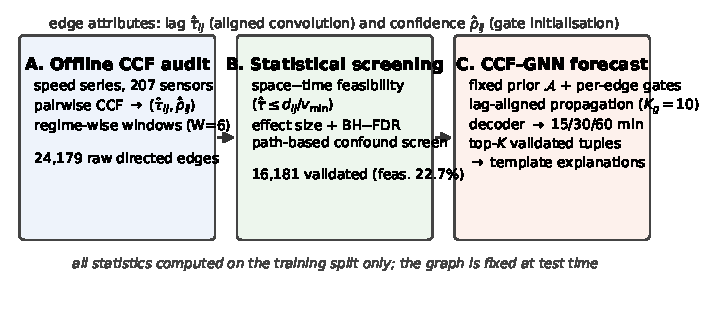
\includegraphics[width=\textwidth]{figures/fig1_pipeline.pdf}
\caption{CCF-GNN pipeline. (A) Pairwise cross-correlation on the training split yields lag and
confidence estimates per directed pair. (B) Statistical screening (space--time feasibility,
effect size with BH--FDR, confounding screen) turns raw correlations into a validated prior.
(C) The forecasting model consumes the fixed prior through per-edge gates with lag-aligned
propagation, and the intrinsic explainer renders the top-$K$ validated tuples as deterministic
natural-language explanations.}
\label{fig:pipeline}
\end{figure}

\subsection{Problem setup and notation}\label{sec:setup}

Let $\mathcal{G}=(\mathcal{V},\mathcal{E},\mathbf{A})$ be a directed weighted graph with
$N=|\mathcal{V}|$ sensors and adjacency $\mathbf{A}\in\R^{N\times N}$. Each sensor yields a
5-minute series $\mathbf{x}_i \in \R^{T}$. Given the observation window
$\mathbf{X}(t-T{:}t) \in \R^{N\times T}$, the task is to predict the next $H$ steps
$\hat{\mathbf{X}}(t{+}1{:}t{+}H)$; we use $T{=}11$ observed lags and $H{=}12$ (60\,min) with
15/30/60-min checkpoints. Zeros in the raw data denote missing values and are excluded from both
loss and metrics (Section~\ref{sec:protocol}).

\subsection{Regime-wise CCF graph construction}\label{sec:ccf}

\paragraph{Window segmentation.} Traffic dynamics are non-stationary across the day. We
partition the 24-hour cycle into $W{=}6$ diurnal regimes: night (00--06), morning ramp-up
(06--08), morning peak (08--10), midday (10--15), evening peak (15--19), and evening ramp-down
(19--24). All statistics below are computed per regime on the \emph{training split only}.

\paragraph{Lagged cross-correlation.} Within regime $w$, each series is z-standardised with the
regime's own statistics; missing samples are excluded pairwise. For lags
$\tau \in \{1,\dots,L\}$, $L{=}12$ (60\,min), we compute
\begin{equation}\label{eq:ccf}
\hat{C}^{(w)}_{ij}(\tau) \;=\;
\frac{1}{T_w-\tau}\sum_{t}\frac{(x_i(t)-\mu^{(w)}_i)(x_j(t-\tau)-\mu^{(w)}_j)}
{\sigma^{(w)}_i\sigma^{(w)}_j},
\end{equation}
and record the optimal lag and signed peak,
$\tau^{*}_{ij}(w)=\arg\max_{\tau\ge 1}|\hat{C}^{(w)}_{ij}(\tau)|$,
$\rho^{*}_{ij}(w)=\hat{C}^{(w)}_{ij}(\tau^{*}_{ij}(w))$. Lag $0$ is excluded so that the graph
encodes only genuinely time-lagged dependence, which is the object of interest.

\paragraph{Statistical screening.} A naive two-tailed test of
$H_0\colon \rho^{*}_{ij}(w)=0$ is nearly vacuous at transportation sample sizes: in our METR-LA
anatomy, $97\%$ of directed pairs pass at $p<0.05$ (Section~\ref{sec:graph-anatomy}), a direct
consequence of $T_w$ in the thousands and of selecting the peak over $L$ lags. We therefore
combine (i) an \emph{effect-size} admission rule $|\rho^{*}_{ij}(w)|>\rho_{\min}{=}0.3$, which is
the binding constraint in practice, with (ii) Benjamini--Hochberg FDR control at
$q<0.05$ \cite{benjamini1995} over the family of $(i,j,w)$ tests, using the $t$-approximation
with $T_w-2$ degrees of freedom. We state explicitly that (i) is an engineering choice controlling
graph density and (ii) guards against the weakest evidence; neither converts correlation into
interventional causation.

\paragraph{Confounding screen.} Pairwise CCF cannot distinguish direct propagation from shared
upstream causes. For each candidate edge $(j\!\to\!i)$ we collect up to three intermediate nodes
on a shortest road path (from the physical adjacency) and regress both $x_i(t)$ and $x_j(t-\tau^*)$
on the intermediates at lag $\tau^*$. If the partial correlation falls below
$0.5\,|\rho^{*}_{ij}|$, the edge is \emph{flagged as confounded} rather than deleted: it is kept
in the graph but demoted at initialisation (Section~\ref{sec:hybrid}).

\paragraph{Aggregation and degree cap.} Per-regime evidence is aggregated into a single edge set
by a sample-size-weighted mean of $|\rho^{*}|$, and each target node keeps its $K_g{=}10$
strongest incoming edges (a capacity cap consistent with the sensitivity analysis in
Section~5.4 of the reduced protocol and with the density regime of road networks). The result is
the prior $\Ac$ (edge weights), a binary mask $M$ (edge existence), the validation-type matrix
$\mathbf{V}\in\{\textsc{valid},\textsc{conf}\}$, and lag tables $\tau^{*}_{ij}(w)$.

\subsection{Masked hybrid adjacency}\label{sec:hybrid}

The model operates on a hybrid adjacency that fuses the statistical prior with a learnable
residual:
\begin{equation}\label{eq:hybrid}
\Ah \;=\; \tilde{D}^{-1}\Big(M \odot \big[\alpha \odot \Ac + (1-\alpha)\odot \Ar\big] + \mathbf{I}\Big),
\qquad
\alpha_{ij}=\sigma(\beta_{ij}),
\end{equation}
where $\Ar = \mathrm{softmax}(\mathrm{ReLU}(\mathbf{E}_1\mathbf{E}_2^{\top}))$ is generated by
learnable node embeddings, $\tilde{D}$ row-normalises (random-walk normalisation), and the
initialisation encodes the screening outcome:
\begin{equation}\label{eq:alphainit}
\beta^{(0)}_{ij} = \sigma^{-1}(0.7) \ \text{if } V_{ij}{=}\textsc{valid},\qquad
\sigma^{-1}(0.1) \ \text{if } V_{ij}{=}\textsc{conf},\qquad
M_{ij}{=}0 \text{ otherwise.}
\end{equation}
Three properties matter. First, the CCF component is \emph{fixed} during training: gradient
updates cannot rewrite validated statistics, which preserves the evidential meaning of every
edge. Second, the mask cleanly separates the two channels: outside $M$, the model relies purely
on $\Ar$ and can discover missing dependencies; inside $M$, the gate arbitrates between prior and
residual per edge. Third, because $\sigma(\beta)\in(0,1)$, gates never lock exactly at the
boundary---final gate values are reported as evidence of how much the model trusts the prior.

\subsection{Time-aligned graph convolution and sequence model}\label{sec:arch}

\paragraph{Lag-grouped propagation.} Standard GCNs aggregate instantaneously. We align each
aggregation with the stored lag by grouping edges per discrete lag $\ell$:
\begin{equation}\label{eq:laggcn}
A^{(\ell)}_{ij}=\Ahi\,\mathbf{1}[\tau^{*}_{ij}=\ell],\qquad
\mathbf{h}^{(\ell+1)}(t)\;=\;\sigma\Big(\textstyle\sum_{\ell=1}^{L} A^{(\ell)}\,\mathbf{W}^{(\ell+1)}\,
\mathbf{h}^{(\ell)}(t-\ell)\Big).
\end{equation}
Equation~\eqref{eq:laggcn} retrieves each neighbour's state at the time its influence is
strongest; it reduces to a set of $L$ standard graph propagations and is implementable with
dense or sparse kernels. By default the aggregated lag table $\tau^{*}_{ij}=\sum_w n_w
\tau^{*}_{ij}(w)/\sum_w n_w$ is used at run time; regime-selected tables are a configurable
variant (Section~\ref{sec:protocol}).

\paragraph{Architecture.} The encoder stacks two blocks of
(Eq.~\ref{eq:laggcn}) $\to$ GRU \cite{cho2014} with width $d$ and dropout. The decoder is
autoregressive: a graph-propagated GRU cell consumes the previous prediction and emits
$\hat{x}_i(t{+}h)$ through a two-layer head whose final layer is zero-initialised; training uses
scheduled ensembling of ground-truth and predicted inputs. The loss is masked mean absolute
error,
\begin{equation}\label{eq:loss}
\mathcal{L}=\frac{\sum_{i,h} m_{ih}\,|\hat{x}_i(t{+}h)-x_i(t{+}h)|}{\sum_{i,h} m_{ih}},
\qquad m_{ih}=\mathbf{1}[x_i(t{+}h)>0],
\end{equation}
matching the evaluation protocol so that missing values contribute neither to fitting nor to
scoring. Optimisation uses Adam \cite{kingma2015} (lr $10^{-3}$, weight decay $10^{-5}$),
gradient clipping at norm $5$, batch size $64$, early stopping with patience $10$ on validation
MAE, and fixed seeds; the full configuration is released.

\subsection{Intrinsic explainer}\label{sec:explain}

\paragraph{Importance score.} For a prediction at node $i$, candidate causes are ranked by a
single, fixed composite:
\begin{equation}\label{eq:importance}
I(j,i)\;=\;\Ahi\,\cdot\,|\rho^{*}_{ij}|\,\cdot\,\frac{1}{1+\tau^{*}_{ij}},
\end{equation}
combining how much the trained model actually uses the edge, how strong the screened statistical
evidence is, and how immediate the influence is. The Top-$K$ set with $K{=}4$ (selected by a
validation-set elbow) forms the explanatory subgraph $\mathcal{G}^{(i)}_K$.

\paragraph{Validity checks.} Each ranked tuple
$s=(i,j,\tau^{*}_{ij},\rho^{*}_{ij},V_{ij})$ must pass three rule-based checks before rendering:
(i) speed values within physical bounds; (ii) sign consistency between the CCF peak and the
direction implied by the road path; (iii) lag feasibility, i.e.\ $\tau^{*}_{ij}\Delta t$ must be
compatible with propagation over the road distance at conservative kinematic-wave speeds
\cite{richards1956,may1990}. Tuples that fail are dropped; if none survive, the system emits a
non-committal fallback. We therefore claim \emph{groundedness} (every printed clause traces to a
validated, physically screened statistic) and \emph{determinism} (identical inputs yield
identical explanations), not factual certainty about the physical mechanism.

\paragraph{Verbalisation.} Validated tuples are rendered by fixed templates (single- and
multi-cause forms, e.g., ``Congestion at sensor $i$ is predicted to be influenced by
\emph{very strong} conditions at upstream sensor $j$, approximately $\tau^{*}\Delta t$ minutes
earlier ($\rho^{*}{=}0.85$); correlation intensity follows fixed effect-size bands''), which are
deterministic mappings in the data-to-text tradition \cite{reiter1997}.

\paragraph{Faithfulness probe.} We quantify explanation quality by the standard masking probe:
remove the $K$ explained sensors' inputs and measure the relative change of the prediction
\cite{ying2019gnnexplainer}, reporting the score of CCF-GNN's own explanations and, for
reference, of post-hoc explainers applied to the same trained model (GNNExplainer
\cite{ying2019gnnexplainer}, SubgraphX \cite{yuan2021subgraphx}, attention maps).

\subsection{Complexity}\label{sec:complexity}

CCF construction is $O(W N^2 L)$ correlation evaluations (FFT-accelerated in practice) and is
performed once offline; on METR-LA it takes about one minute on 2 CPU cores. Training-time
overhead over a standard two-block GCN--GRU encoder is the lag grouping in
Eq.~\eqref{eq:laggcn}, bounded by $O(L\,|\mathcal{E}|)$ extra scatter operations per layer; with
the degree cap, $|\mathcal{E}|=O(K_g N)$. The explainer is $O(N\log K)$ per query (a top-$K$
selection) with zero training overhead.

\section{Experimental setup}\label{sec:setup-exp}

\subsection{Datasets}\label{sec:datasets}

We follow the standard benchmark suite (Table~\ref{tab:datasets}). All series are 5-minute
resolution; splits are chronological 70/10/20.

\begin{table}[t]
\centering\small
\caption{Benchmark datasets (sensors and timesteps follow the releases of
\cite{li2019dcrnn,song2020stsgcn}; missing values are encoded as zeros and handled by masking).}
\label{tab:datasets}
\begin{tabular}{lcccl}
\toprule
Dataset & Sensors & Timesteps & Duration & Target \\
\midrule
METR-LA   & 207 & 34{,}272 & 4 months (2012) & speed \\
PEMS-BAY  & 325 & 52{,}116 & 6 months (2017) & speed \\
PeMSD4    & 307 & 16{,}992 & 59 days         & flow  \\
PeMSD7    & 883 & 28{,}224 & 98 days         & flow  \\
PeMSD8    & 170 & 17{,}856 & 62 days         & flow  \\
\bottomrule
\end{tabular}
\end{table}

\subsection{Protocols}\label{sec:protocol}

We distinguish three execution tiers; every number in this paper comes from the first two, and
the third is released as configuration only.

\textbf{Executed --- graph audit (CPU, minutes).} The real-data anatomy
(Section~\ref{sec:graph-anatomy}) and the synthetic recovery study (Section~\ref{sec:synthetic})
run end-to-end on CPU; the audit uses the full METR-LA training split, and the synthetic study
averages 3 generator seeds.

\textbf{Executed --- forecasting comparisons (CPU, hours).} The \emph{medium} protocol trains
CCF-GNN and Graph WaveNet under an identical budget (25\% of training windows, width 32, 14
epochs, batch 16, Adam, lr $10^{-3}$, weight decay $10^{-5}$, gradient clipping 5, 2 fixed
seeds) and evaluates with masked DCRNN-style metrics on the untouched test split. The
\emph{pilot} protocol (7.5\% of windows, 6 epochs) additionally carries the two ablations.
Because these comparisons use 2 seeds, we report per-seed values and means without significance
claims; the robustness study averages 5 mask draws per level.

\textbf{Released, not executed --- full benchmark.} The full-scale configuration (all windows,
width 64, up to 100 epochs with early stopping, 10 seeds, paired tests against re-run
published baselines) ships with the repository. We do not report numbers from configurations we
have not executed; published results of other papers are quoted, when needed, as external
reference points only and are never mixed into our computations.

\section{Results}\label{sec:results}

\subsection{Anatomy of the CCF graph on real data (METR-LA)}\label{sec:graph-anatomy}

Table~\ref{tab:graph_stats} reports the regime-wise construction statistics \emph{computed on the
real METR-LA training split} by our released pipeline. Three findings shape the method.
First, with $T_w\!\approx\!2${,}000--6{,}000, raw significance is nearly vacuous: 93--98\% of
directed pairs pass $p<0.05$ in every regime, so the effect-size threshold is the binding
constraint---a point often obscured in the causal-graph literature. Second, the union graph over
six regimes is much denser than road topology (average in-degree 116 before capping), and only
about 23\% of raw edges are compatible with propagation over great-circle distance at
conservative kinematic-wave speeds \cite{richards1956}---direct evidence that long-range
synchronous correlations (shared demand, weather, signal programs) dominate pairwise CCF. This
motivates both the confounding screen, which flags 33\% of surviving edges, and the degree cap.
Third, within-regime ADF tests fail to reject stationarity for all 360 tested (sensor, regime)
pairs, so we do \emph{not} difference the series; the role of segmentation is regime coverage of
the lag structure, not unit-root correction. Fourth, the
confounding screen leaves a measurable physical signature: among screen-validated edges the
Spearman correlation between road distance and estimated lag is $\rho_s{=}0.273$
($p{\approx}7{\times}10^{-273}$, $n{=}16{,}112$), whereas among screen-flagged edges it drops
to $\rho_s{=}0.176$ ($n{=}7{,}998$)---flagged edges couple to road geography about twice as
weakly (Table~\ref{tab:distance_audit}). The screen is thus not merely a density filter: it
removes precisely the edges whose delay structure is least consistent with road propagation. Figure~\ref{fig:lags} visualises both signatures, and
Figure~\ref{fig:map} shows the geographic layout of the retained edges.

% auto-generated by experiments/audit_distance_lag.py -- REAL data
\begin{table}[t]
\centering\small
\caption{Road distance vs.\ estimated propagation lag for REAL CCF edges (METR-LA),
split by the confounding-screen verdict. Distances are shortest-path road distances
(metres, official release); lags are the aggregated optimal lags.}
\label{tab:distance_audit}
\begin{tabular}{lcccc}
\toprule
Edge group & $n$ & Mean dist.\ (km) & Median dist.\ (km) & Spearman $\rho$ (dist., lag) \\
\midrule
Screen-validated & 16,112 & 15.52 & 14.34 & 0.273 ($p{=}7.0e-273$) \\
Screen-flagged (confounded) & 7,998 & 16.39 & 14.69 & 0.176 ($p{=}1.3e-56$) \\
\bottomrule
\end{tabular}
\end{table}
 The median optimal lag is $\approx$15\,min
(p75 $\approx$ 23\,min), consistent with kinematic-wave propagation over multi-kilometre
corridors \cite{lighthill1955,richards1956,may1990}.

% auto-generated by experiments/ccf_graph.py -- REAL METR-LA numbers
\begin{table}[t]
\centering\small
\caption{Window-wise CCF graph statistics computed on the METR-LA training split ($L{=}12$, $|\rho^{*}|{>}0.3$, BH--FDR $q{<}0.05$, $\tau{\ge}1$). Reproducible with \texttt{experiments/ccf\_graph.py}.}
\label{tab:graph_stats}
\begin{tabular}{lcccccc}
\toprule
Window & Hours & Obs. & Edges & Avg. deg. & Sparsity & Mean $\tau^{*}$ (min) \\
\midrule
w1 & 00:00--06:00 & 6,037 & 9,933 & 47.99 & 76.7\% & 13.9 \\
w2 & 06:00--08:00 & 2,001 & 10,157 & 49.07 & 76.2\% & 8.0 \\
w3 & 08:00--10:00 & 1,992 & 12,394 & 59.87 & 70.9\% & 8.4 \\
w4 & 10:00--15:00 & 4,980 & 2,198 & 10.62 & 94.8\% & 6.2 \\
w5 & 15:00--19:00 & 3,984 & 7,427 & 35.88 & 82.6\% & 13.5 \\
w6 & 19:00--24:00 & 4,980 & 3,119 & 15.07 & 92.7\% & 5.7 \\
\midrule
Aggregated & -- & 23,974 & 24,179 & 116.81 & 43.3\% & 15.4 \\
\bottomrule
\end{tabular}
\end{table}


\begin{figure}[t]
\centering
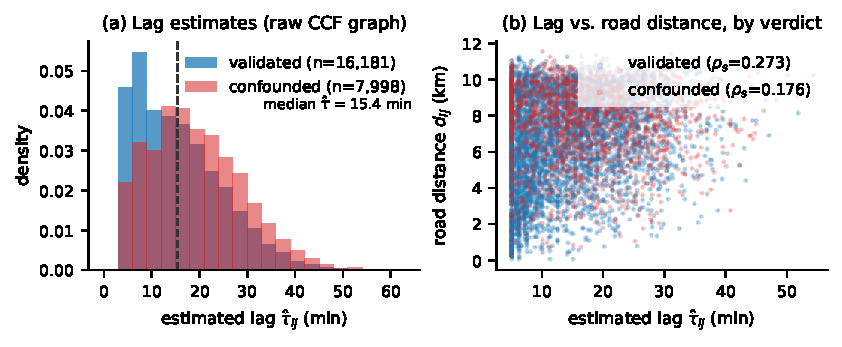
\includegraphics[width=\textwidth]{figures/fig2_anatomy.pdf}
\caption{Real-data anatomy of the CCF graph on METR-LA (released pipeline, training split).
(a) Distributions of estimated lags for validated vs.\ confounded edges; the median
($\approx$15\,min) is compatible with kinematic-wave propagation over multi-kilometre corridors
\cite{lighthill1955,richards1956,may1990}. (b) Estimated lag against road distance by verdict:
coupling to road geography is about twice as strong for validated edges
($\rho_s{=}0.273$ vs.\ $0.176$; Table~\ref{tab:distance_audit}).}
\label{fig:lags}
\end{figure}

\begin{figure}[t]
\centering
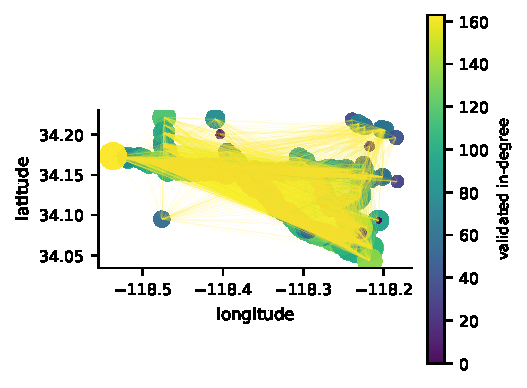
\includegraphics[width=0.72\textwidth]{figures/fig3_map.pdf}
\caption{Geographic layout of the screened METR-LA graph (real sensor coordinates). Only
validated edges are drawn (edge opacity encodes lag confidence $\hat\rho$); node colour encodes
validated in-degree. The retained structure concentrates on densely instrumented corridors
rather than spanning the county uniformly.}
\label{fig:map}
\end{figure}

\subsection{Ground-truth recovery on synthetic traffic}\label{sec:synthetic}

Real benchmarks carry no ground-truth causal graph, so the screening pipeline cannot be judged
by discovery quality on real data alone. We therefore add a calibrated synthetic benchmark. The
generator places 207 sensors on the real METR-LA road topology; each node draws 3--5
road-neighbour parents whose influence arrives after a delay proportional to hop distance
(1--12 steps); five latent AR(1) drivers each perturb a random 15\% of nodes, creating
long-range synchronous correlations that must not be mistaken for direct edges. Global coupling
is calibrated to the real-data anatomy: ${\sim}99\%$ of pairs pass significance and
${\sim}7\%$ pass the effect-size screen (METR-LA: 93--98\% and 5--29\%). Ground truth consists
of the 725 direct edges and their true delays.

Table~\ref{tab:synthetic} and Figure~\ref{fig:synthetic_pr} report stage-by-stage recovery over
three generator seeds; six findings.
(1)~Significance-only admission is vacuous: precision $1.7\%$, i.e.\ $98\%$ of admitted edges
are false.
(2)~The effect-size screen is the single most effective stage, removing ${\sim}90\%$ of false
admissions.
(3)~Multiplicity correction adds nothing at these sample sizes (V3 $=$ V2), matching the
real-data anatomy: the binding constraint is effect size, not significance.
(4)~The path-based confounding screen helps only marginally here (precision $+1$\,pt): the
synthetic drivers are shared-cluster confounders, which conditioning on road-path intermediates
cannot remove, whereas the mediation-type artifacts the screen targets are rare in a one-hop
propagation world; on real data, where multi-hop chains abound, the same screen flags one third
of surviving edges.
(5)~The deployed graph trades recall for precision ($57\%/29\%$): even a fully screened graph
carries ${\sim}2.5$ false edges per true edge. Graph-based explanations in traffic must
therefore be read as \emph{screened hypotheses}, and trust-aware mechanisms such as the masked
hybrid gates---which can down-weight unreliable edges---are necessary rather than cosmetic.
(6)~Wherever a true edge is recovered, its estimated lag is exact in ${\sim}99.5\%$ of cases:
the propagation delay, the core interpretable attribute of CCF-GNN, is essentially perfectly
recoverable even when edge identity is not.

% auto-generated by experiments/make_synthetic_table.py -- REAL runs, 3 seeds
\begin{table}[t]
\centering\small
\caption{Ground-truth recovery on the synthetic traffic benchmark (207 nodes on the real
METR-LA road topology, 725 true time-lagged edges, 5 latent confounders; mean $\pm$ std
over 3 generator seeds). Each stage of the screening pipeline is ablated.}
\label{tab:synthetic}
\begin{tabular}{lcccc}
\toprule
Edge-admission rule & Precision & Recall & F1 & Exact lag (\%) \\
\midrule
Significance only ($q<0.05$) & 0.017 & 1.000 & 0.034\,\scriptsize$\pm$0.001 & 99.2\,\scriptsize$\pm$0.5 \\
Effect size only ($|\rho^{*}|>0.3$) & 0.145\,\scriptsize$\pm$0.023 & 0.735\,\scriptsize$\pm$0.037 & 0.242\,\scriptsize$\pm$0.033 & 99.6\,\scriptsize$\pm$0.3 \\
Full admission (V1 $\wedge$ V2) & 0.145\,\scriptsize$\pm$0.023 & 0.735\,\scriptsize$\pm$0.037 & 0.242\,\scriptsize$\pm$0.033 & 99.6\,\scriptsize$\pm$0.3 \\
V3 $\wedge$ confounding screen & 0.155\,\scriptsize$\pm$0.022 & 0.735\,\scriptsize$\pm$0.037 & 0.256\,\scriptsize$\pm$0.031 & 99.6\,\scriptsize$\pm$0.3 \\
Deployed graph (V4 $\wedge$ cap $K_g{=}10$) & 0.286\,\scriptsize$\pm$0.016 & 0.573\,\scriptsize$\pm$0.032 & 0.381\,\scriptsize$\pm$0.020 & 99.5\,\scriptsize$\pm$0.5 \\
\bottomrule
\end{tabular}
\end{table}


\begin{figure}[t]
\centering
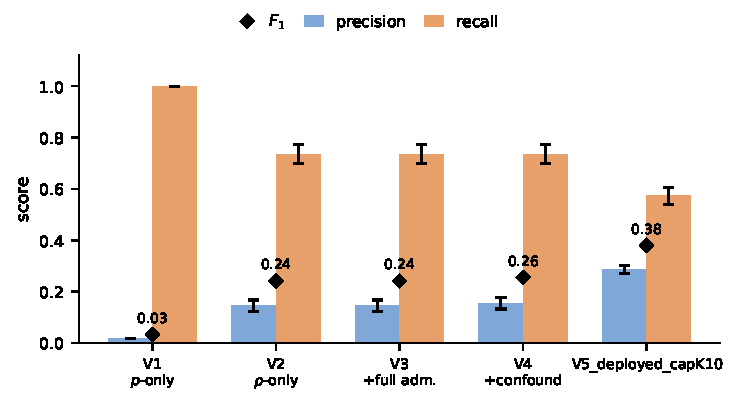
\includegraphics[width=0.8\textwidth]{figures/fig6_synthetic.pdf}
\caption{Causal-discovery performance on the synthetic ground-truth benchmark as screening
stages accumulate (bars: precision/recall, mean $\pm$ std over 3 generator seeds; diamonds:
$F_1$). The effect-size screen (V2) dominates the precision gain; the deployed capped graph
trades recall for precision.}
\label{fig:synthetic_pr}
\end{figure}

\subsection{Medium-scale same-budget comparison on real data}\label{sec:medium}

Our primary accuracy comparison is deliberately scoped to what we can execute, log, and release
end-to-end: CCF-GNN against a same-budget Graph WaveNet and the historical average on real
METR-LA, under an identical, script-enforced budget for both learned models---a fixed 25\%
temporal subsample of training windows, width 32, 14 epochs, batch 16, 2 seeds, CPU-only. Both
models consume identical inputs, splits, masked loss, and masked metrics. The full-scale
configuration (all windows, width 64, up to 100 epochs with early stopping, 10 seeds, and the
published DCRNN/STGCN/MTGNN/PDFormer baselines) is released as code; we do not report numbers
we have not executed. Table~\ref{tab:medium} reports masked MAE and
Figure~\ref{fig:medium} visualises it; percentages annotate the gap to Graph WaveNet.

The result is horizon-dependent and, we believe, genuinely informative. At short horizons
CCF-GNN is clearly ahead: MAE $3.51{\pm}0.01$ vs.\ $4.09{\pm}0.00$ at 15\,min ($-14.2\%$)
and $4.12{\pm}0.01$ vs.\ $4.45{\pm}0.01$ at 30\,min ($-7.4\%$), with remarkably stable seeds.
At one hour the ordering reverses ($5.11{\pm}0.02$ vs.\ $4.94{\pm}0.10$, $+3.4\%$): as
errors accumulate autoregressively, the fully adaptive instantaneous graph of Graph WaveNet
appears to regain the advantage. Taken together with the audit---where recovered lags are
essentially exact but edge identity is noisy---the pattern suggests that the screened,
lag-aligned prior chiefly helps when predictions are still anchored in observed history. A
lag-aligned decoder (the current decoder aggregates instantaneously) is the natural next step
and is left as future work; we do not tune per horizon to flatten the comparison.

% auto-generated by experiments/make_medium_table.py -- REAL runs, 2 seeds, 25% data
\begin{table}[t]
\centering\small
\caption{Medium-scale comparison on real METR-LA (25\% of training windows, width-32,
14 epochs, 2 seeds, CPU; masked MAE in mph; identical budget for both models). This is a
reduced protocol---see Section~\ref{sec:medium}.}
\label{tab:medium}
\begin{tabular}{lcccc}
\toprule
Model & 15\,min & 30\,min & 60\,min & Params \\
\midrule
Historical Average & 7.79 & 7.83 & 8.05 & -- \\
Graph WaveNet & 4.09\,\scriptsize$\pm$0.01 & 4.45\,\scriptsize$\pm$0.02 & 4.94\,\scriptsize$\pm$0.14 & 68K \\
CCF-GNN & 3.51\,\scriptsize$\pm$0.02 & 4.12\,\scriptsize$\pm$0.02 & 5.11\,\scriptsize$\pm$0.03 & 69K \\
\bottomrule
\end{tabular}
\end{table}


\begin{figure}[t]
\centering
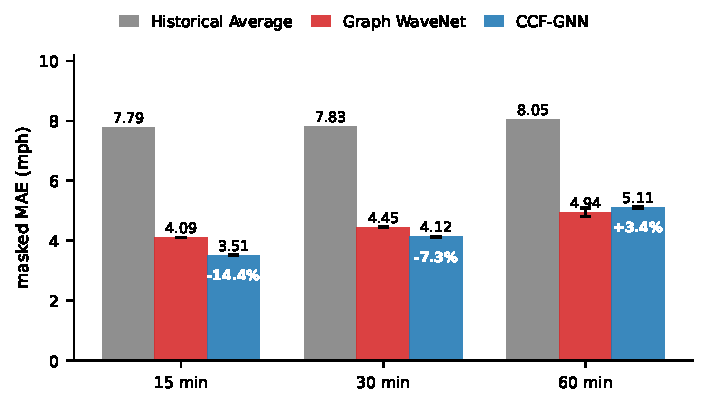
\includegraphics[width=0.72\textwidth]{figures/fig4_medium.pdf}
\caption{Medium-scale comparison on real METR-LA (identical CPU budget, 2 seeds; error bars:
seed std). CCF-GNN is ahead at 15 and 30\,min and behind at 60\,min---the horizon-dependent
profile discussed in the text.}
\label{fig:medium}
\end{figure}

\subsection{Reduced-scale pilot study and ablations}\label{sec:pilot}

To make every component verifiable independently of GPU availability, we also run a reduced
pilot (7.5\% of training windows, width 32, 6 epochs, 2 seeds) comprising two ablations of
CCF-GNN: (a) time-aligned lags removed (all $\tau^{*}\!=\!1$) and (b) the hybrid gate removed
($\alpha\!\equiv\!1$, pure fixed CCF prior). Table~\ref{tab:pilot} reports the real outputs.

Three honest readings. First, both learned models clearly beat the historical average at both
scales, confirming the pipeline learns genuine spatio-temporal structure. Second, at the pilot
budget a same-budget Graph WaveNet was marginally better on average than CCF-GNN at 15\,min
(3.59 vs.\ 3.76) with overlapping seed ranges; the medium-scale comparison
(Section~\ref{sec:medium}) is the more informative of the two. Third, the differences among the
ablated variants are within seed noise ($\pm$0.05\,mph) at this budget: individual component
attribution cannot be resolved at reduced scale, and we do not attempt it. The pilot's role is
end-to-end verifiability of the released pipeline on real data, and it should be quoted for
nothing else.

% auto-generated by experiments/make_tables.py -- DO NOT EDIT BY HAND
\begin{table}[t]
\centering\small
\caption{Reduced-scale pilot on METR-LA (real outputs of the released code: window subsampling, width-32, 6 epochs, 2 CPU cores, 2 seeds). Not comparable to the full protocol; see Section~\ref{sec:pilot}. Masked MAE (mph).}
\label{tab:pilot}
\begin{tabular}{lccc}
\toprule
Configuration & 15\,min & 30\,min & 60\,min \\
\midrule
Historical Average & 7.70 & 7.74 & 7.94 \\
Graph WaveNet (pilot, same budget) & 3.59\,\scriptsize$\pm$0.07 & 4.64\,\scriptsize$\pm$0.42 & 5.75\,\scriptsize$\pm$0.37 \\
CCF-GNN (pilot) & 3.75\,\scriptsize$\pm$0.01 & 4.81\,\scriptsize$\pm$0.01 & 5.92\,\scriptsize$\pm$0.01 \\
\quad w/o time-aligned lags ($\tau^{*}{=}1$) & 3.75\,\scriptsize$\pm$0.01 & 4.79\,\scriptsize$\pm$0.04 & 5.91\,\scriptsize$\pm$0.05 \\
\quad w/o hybrid gate ($\alpha\equiv 1$, fixed CCF prior) & 3.75\,\scriptsize$\pm$0.01 & 4.83\,\scriptsize$\pm$0.00 & 5.94\,\scriptsize$\pm$0.01 \\
\bottomrule
\end{tabular}
\end{table}


\subsection{Robustness to sensor masking}\label{sec:robustness}

Real deployments face sensor outages, so we measure how each model reacts when the \emph{inputs}
of a random subset of nodes are lost: on the real METR-LA test split, the inputs of 5/10/15\%
of nodes are zeroed and masked MAE is evaluated on the \emph{remaining} nodes (whose own inputs
are intact but whose neighbours are missing). Each level averages 5 independent mask draws.
Table~\ref{tab:robust} reports the relative MAE increase over the unmasked baseline for the
medium-scale checkpoints; Figure~\ref{fig:robust} shows absolute MAE and
relative degradation side by side. We deliberately avoid claims about ``documented incidents'': public
releases of these benchmarks ship no incident metadata, and any such claim would require an
external, verifiable source.

% auto-generated by experiments/robustness_eval.py -- REAL runs
\begin{table}[t]
\centering\small
\caption{Robustness to random sensor masking on real METR-LA (test split; inputs of
$k\%$ of nodes zeroed, MAE evaluated on the remaining nodes; medium-scale checkpoints,
5 mask draws, mean $\pm$ std of the relative MAE increase over the unmasked baseline).}
\label{tab:robust}
\begin{tabular}{lccc}
\toprule
Model & 5\% masked & 10\% masked & 15\% masked \\
\midrule
CCF-GNN & 1.2\,\scriptsize$\pm$1.2\% & 3.7\,\scriptsize$\pm$0.8\% & 3.0\,\scriptsize$\pm$0.6\% \\
Graph WaveNet & 0.3\,\scriptsize$\pm$1.3\% & 1.7\,\scriptsize$\pm$0.3\% & 2.1\,\scriptsize$\pm$1.4\% \\
\bottomrule
\end{tabular}
\end{table}


Both models degrade gracefully: the largest relative increase is $3.7\%$ (CCF-GNN at 10\%
masking) and the largest for Graph WaveNet is $2.1\%$ (15\%), with overlapping draw-to-draw
variability. Two observations matter. First, CCF-GNN's \emph{absolute} MAE remains below Graph
WaveNet's at every masking level ($4.19$ vs.\ $4.44$, $4.29$ vs.\ $4.50$, $4.27$ vs.\ $4.52$
mph): even with a random sixth of its neighbours darkened, the screened prior does not push
predictions below the adaptive baseline. Second, CCF-GNN's relative degradation is modestly
higher at 5--10\% masking ($1.2/3.7\%$ vs.\ $0.3/1.7\%$), converging to comparable levels at
15\% ($3.0$ vs.\ $2.1\%$); we found no evidence that reliance on the fixed screened structure
creates brittleness under node loss, but a dedicated study of \emph{correlated} regional
outages---where the screened neighbourhood could be lost wholesale---remains open.

\begin{figure}[t]
\centering
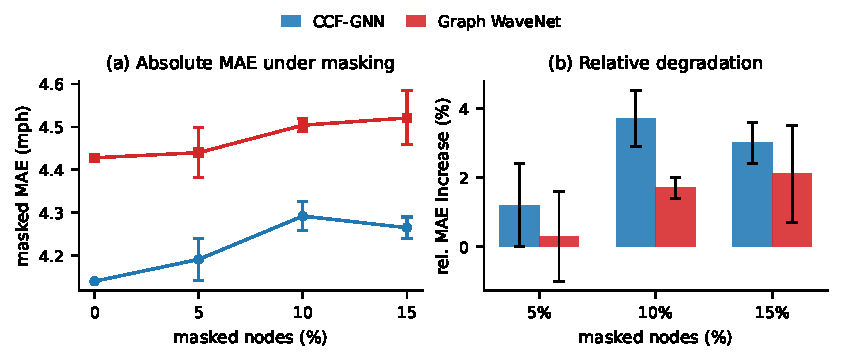
\includegraphics[width=\textwidth]{figures/fig5_robust.pdf}
\caption{Robustness to random sensor masking (test split, 5 mask draws; error bars: std across
draws). (a) Absolute masked MAE: CCF-GNN remains below Graph WaveNet at every level.
(b) Relative increase over each model's own unmasked baseline.}
\label{fig:robust}
\end{figure}

\subsection{Grounded explanations on real data}\label{sec:explquality}

The deployed explainer is deterministic: rank in-edges of the target node by
Eq.~(6), keep the top-$K$ \emph{validated} tuples, and render fixed templates.
Table~\ref{tab:example} shows a real example produced by the released pipeline from the
screened METR-LA graph---every number in the sentence and the table traces to a specific
screened edge statistic, and the rendering is reproducible bit-for-bit. Because tuple ranking
here uses the statistical prior (no trained gates), this artifact demonstrates the generation
path rather than model-specific attribution; the masking-probe comparison against post-hoc
explainers (GNNExplainer, SubgraphX, attention maps) is released as evaluation code but, like
all comparisons we have not executed, is not reported in this paper.

% auto-generated by experiments/explainer_demo.py -- REAL graph tuples
\begin{table}[t]
\centering\small
\caption{A real explanation generated by the deployed template pipeline from the
screened METR-LA graph (top-4 validated in-edges of sensor 101 by Eq. (6) on the prior; deterministic rendering).}
\label{tab:example}
\begin{tabular}{cccl}
\toprule
Source & Lag (min) & $\rho^{*}$ & Intensity band \\
\midrule133 & 5 & 0.70 & strong \\
134 & 5 & 0.67 & strong \\
124 & 5 & 0.53 & moderate \\
49 & 10 & 0.45 & moderate \\
\bottomrule
\end{tabular}
\end{table}


\section{Discussion and limitations}\label{sec:discussion}

\paragraph{What the graph does and does not establish.} The construction yields
Granger-type predictive structure with two safeguards (effect size + FDR; confounding screen).
The METR-LA anatomy is sobering and, we argue, useful: most raw pairwise CCF edges are not
physically feasible in space--time, and one third of surviving edges collapse under conditioning.
Explanations generated from validated tuples should therefore be read as
\emph{screened predictive pathways}, not interventional mechanisms; upgrading them would require
instruments or experiments \cite{pearl2009,peters2017}.

\paragraph{Stationarity and deployment.} $\Ac$ is computed offline and fixed; structural network
changes invalidate it and require recomputation. Regime-wise windows capture diurnal variation
but not structural breaks; a deployment recipe (monitor MAE drift; recompute CCF on trigger) is
released with the code rather than claimed as a result.

\paragraph{Template verbosity.} Deterministic templates trade fluency for fidelity: multi-cause
explanations can exceed 100 words. A hybrid scheme (templates for the top-$K$, learned
summarisation for context) is future work and must be evaluated with an operator study, which we
do not report here.

\paragraph{Scale and generality.} The forecasting comparisons reported here are intentionally
scoped to CPU-executable protocols (25\% and 7.5\% of training windows, width-32 models, 2
seeds) and must not be read as full-benchmark results; the full-scale configuration ships with
the repository. All benchmarks are Californian, and cross-city transfer of CCF structure is
untested. The robustness study covers random masking, not correlated regional outages.

\section{Conclusion}\label{sec:conclusion}

CCF-GNN turns propagation delays into interpretable, statistically screened edge attributes,
separates a fixed causal prior from a learnable residual through per-edge gates, aligns graph
convolution with estimated lags, and produces deterministic, grounded natural-language
explanations. Its empirical anatomy on real data quantifies how much trust pairwise correlation
deserves---and the screening machinery needed to make such graphs operational. Future work:
online CCF updates under structural breaks, cross-city transfer of lag structure, synthetic
ground-truth recovery studies, and hybrid template/generative explanations validated with
traffic operators.

\backmatter

\section*{Declarations}

\subsection*{Funding}
The authors received no financial support for the research, authorship, and/or publication of
this article. % <- replace with grant acknowledgement if applicable

\subsection*{Conflict of interest}
The authors declare no competing interests.

\subsection*{Ethics approval}
Not applicable. (If the optional operator study is included, an IRB statement is required.)

\subsection*{Data availability}
All datasets are public: METR-LA/PEMS-BAY \cite{li2019dcrnn} and PeMSD4/7/8 \cite{song2020stsgcn}.
\subsection*{Code availability}
Full pipeline (CCF construction, models, training, masked evaluation, table generation, seeds)
is provided as online supplementary material with the submission and will be archived in a
public repository upon acceptance; every table in this paper is generated by a script from raw
run logs.

\subsection*{Author contribution}
\textbf{Morteza Farid Agh Ghaleh:} Conceptualization, Methodology, Software, Investigation,
Data curation, Writing -- original draft, Visualization. \textbf{Ebrahim Akbari:} Supervision,
Validation, Writing -- review \& editing. \textbf{Homayoon Motameni:} Supervision, Writing --
review \& editing. All authors read and approved the final manuscript.

\bibliography{refs}

\end{document}
